%%This is a skeleton file for writing an e-lab paper (University College of Antwerp)
%%Both this file and the accompanying elab.cls file are the worj of Michael Shell (IEEETran)
%%All credit goes to him!


%% Support sites:
%% http://www.michaelshell.org/tex/ieeetran/
%% http://www.ctan.org/tex-archive/macros/latex/contrib/IEEEtran/
%% and
%% http://www.ieee.org/


\documentclass[9pt,journal,compsoc,twoside, a4paper]{elab}



% Some very useful LaTeX packages include:


% *** GRAPHICS RELATED PACKAGES ***
\usepackage[pdftex]{graphicx}
% http://www.ctan.org/tex-archive/macros/latex/required/graphics/
% Another good source of documentation is "Using Imported Graphics in
% LaTeX2e" by Keith Reckdahl which can be found as epslatex.ps or
% epslatex.pdf at: http://www.ctan.org/tex-archive/info/
%
% latex, and pdflatex in dvi mode, support graphics in encapsulated
% postscript (.eps) format. pdflatex in pdf mode supports graphics
% in .pdf, .jpeg, .png and .mps (metapost) formats. Users should ensure
% that all non-photo figures use a vector format (.eps, .pdf, .mps) and
% not a bitmapped formats (.jpeg, .png).

% *** MATH PACKAGES ***
\usepackage[cmex10]{amsmath}
% A popular package from the American Mathematical Society that provides
% many useful and powerful commands for dealing with mathematics.
% http://www.ctan.org/tex-archive/macros/latex/required/amslatex/math/

% *** SPECIALIZED LIST PACKAGES ***
\usepackage{algorithmic}
% algorithmic.sty was written by Peter Williams and Rogerio Brito.
% This package provides an algorithmic environment fo describing algorithms.
% You can use the algorithmic environment in-text or within a figure
% environment to provide for a floating algorithm. Do NOT use the algorithm
% floating environment provided by algorithm.sty (by the same authors) or
% algorithm2e.sty (by Christophe Fiorio) 
% http://www.ctan.org/tex-archive/macros/latex/contrib/algorithms/
% There is also a support site at:
% http://algorithms.berlios.de/index.html

% *** SUBFIGURE PACKAGES ***
\usepackage[tight,normalsize,sf,SF]{subfigure}
% subfigure.sty was written by Steven Douglas Cochran. This package makes it
% easy to put subfigures in your figures. e.g., "Figure 1a and 1b". 
% http://www.ctan.org/tex-archive/obsolete/macros/latex/contrib/subfigure/
% subfigure.sty has been superceeded by subfig.sty.


% *** PDF, URL AND HYPERLINK PACKAGES ***
\usepackage{url}
% url.sty was written by Donald Arseneau. It provides better support for
% handling and breaking URLs. url.sty is already installed on most LaTeX
% systems. The latest version can be obtained at:
% http://www.ctan.org/tex-archive/macros/latex/contrib/misc/
% Read the url.sty source comments for usage information. Basically,
% \url{my_url_here}.


% *** Do not adjust lengths that control margins, column widths, etc. ***
% *** Do not use packages that alter fonts (such as pslatex).         ***

% correct bad hyphenation here
\hyphenation{op-tical net-works semi-conduc-tor}
% Declare graphics path


\begin{document}

% paper title
% can use linebreaks \\ within to get better formatting as desired
\title{An implementation of the \\Filtered Back Projection algorithm using Matlab}


\author
{
		Tim~Schaeps,
    Maggie~Goossens,
    Joost~Batenburg,
    Jan Sijbers,
    and~Tim Dams.% <-this % stops a space
		\IEEEcompsocitemizethanks
		{
			\IEEEcompsocthanksitem T. Schaeps, M. Goossens and T. Dams are with the University 	College of Antwerp, Paardenmarkt 92, 2000 Antwerp, Belgium\protect\\
			% note need leading \protect in front of \\ to get a newline within \thanks as
			E-mail: see http://www.e-lab.be
			\IEEEcompsocthanksitem K.J. Batenburg and Jan Sijbers are with the University of Antwerp
		}% <-this % stops a space
		\thanks{Manuscript received June, 2007; revised September 11, 2007.}
}


% The paper headers %Leave like this!
\markboth{Papers of the e-lab master theses' 2007-2008}%
{FBP algorithm using Matlab}

% The only time the second header will appear is for the odd numbered pages
% after the title page when using the twoside option.

\IEEEcompsoctitleabstractindextext{%
\begin{abstract}
Tomography is a technique developed with the purpose of getting structural information out of an object as realistic as possible without opening the object.  Evidently one cannot take just a picture. With the use of several types of scanners, data needed to reconstruct this information is delivered. There are several ways to achieve this, but one of them, the filtered back projection algorithm, will be discussed in this paper. The goal is to give a representation of the original internal structure. Different possibilities for implementation will be taken into account with the purpose of giving a detailed overview of this technique.
\end{abstract}

\begin{IEEEkeywords}
filter back projection, tomography, medical imaging, matlab.
\end{IEEEkeywords}}


% make the title area
\maketitle
\IEEEdisplaynotcompsoctitleabstractindextext

%Leave this part alone, it is pretty fragile!
  \noindent\raisebox{2\baselineskip}[0pt][0pt]%
  {\parbox{\columnwidth}{\section{Introduction}\label{sec:introduction}%
  \global\everypar=\everypar}}%
  \vspace{-1\baselineskip}\vspace{-\parskip}\par


%Now starts your actual paper. Only the first letter of the Introduction needs a larger, so-called
%drop letter. ALL OTHER SECTIONS/SUBSECTIONS START WITH A NORMAL LETTER.

% form to use if the first word consists of a single letter:
% \IEEEPARstart{A}{demo} file is ....
% 
% form to use if you need the single drop letter followed by
% normal text (unknown if ever used by IEEE):
% \IEEEPARstart{A}{}demo file is ....

% You must have at least 2 lines in the paragraph with the drop letter
% (should never be an issue)

% Here we have the typical use of a "T" for an initial drop letter
% and "omography" in caps to complete the first word.
\IEEEPARstart{T}{omography} is a technique used to get an overview of structures inside for example a human body or non biological object without the need to open the object. One can also say that this is a nondestructive way of obtaining visual data from the inside of an object. When an X-ray scanner makes projections at different angles around the object, the data obtained using this process have to be reconstructed in one way or another. The data without reconstruction are meaningless. \cite{POCT1} describes all the essential factors that have to be taken into account.
One technique to achieve this is the filtered back projection (FBP) method. It is based on the Back Projection (BP) algorithm \cite{Anastasio2001}. BP is not exact and the reconstructed image is blurry. This is a reason why this technique isn't qualified for clinical applications. That is where FBP comes in: Projected data are filtered and  "smeared" out at the same angles at which the projections were taken. FBP is a very popular technique that is still preferred over relatively young and promising iterative techniques such as ART \cite{Frederik1999}.  We also need to consider the intended quality of the reconstructed image. The size of angles at which the projections were made during a CT-scan determines the quality of the reconstructed image. When a big angle ($\theta$) between projections is used, for example (e.g. $\pi$/18 rad) there are fewer projections than when a smaller angle is used (e.g. $\pi$/90 rad).  This can also be seen in figure \ref{fig:Projections}.


%An example of a figure inclusion. Always make sure there is at least one reference to the image in your text. 
\begin{figure}[hbt]
	\centering
		\subfigure[][10 Projections]{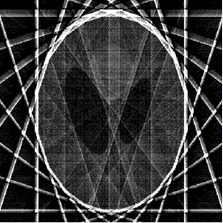
\includegraphics[width=0.24\textwidth,keepaspectratio]{Images/img1.png}}
		\subfigure[][100 Projections]{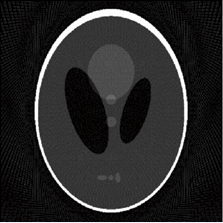
\includegraphics[width=0.24\textwidth,keepaspectratio]{Images/img2.png}}
		\caption{Difference between different amounts of projections}
	\label{fig:Projections}
\end{figure}
It is evident that the latter method, using smaller angles, gives a far better result than the first one, because there are more projections and as a result more detail in the final image. The counter side however is the fact that a smaller angle also results in more data and thus more computing time needed. Considering this, we need to decide whether quality is more important, or fast visualization. This decision can be made case by case. There are still other possibilities available, which will be discussed together with the technique in detail further on. 

\subsection{Main goal}
The main goal of this research was to create an all-in application, which gives an overview of the complete process of image-data acquisition of an object. There are several techniques available. In this paper the FBP method will be discussed. Using Matlab, this method will be implemented in a toolbox which has an educational purpose. To achieve a maximal overview, the different steps in the project will be developed and discussed in modules.  These modules will be discussed in detail in the next section.


\subsubsection{Theory}

A solid mathematical foundation is obtained through the following explanation \cite{POCT1}. First we consider a coordinate system (t,s) to be a rotated version of the well known original (x,y) system.

%Here we add an equation
\begin{equation}
\label{rotationformula}
\left[ \begin{array}{l}
 x2 \\ 
 y2 \\ 
 \end{array} \right] = \left[ \begin{array}{l}
 \cos (\theta) \\ 
 \sin (\theta) \\ 
 \end{array} \right.\left. \begin{array}{l}
  -\sin (\theta) \\ 
 \cos (\theta) \\ 
 \end{array} \right]*\left[ \begin{array}{l}
 x1 \\ 
 y1 \\ 
 \end{array} \right]
%%\]
\end{equation}	
%
\par A projection along lines of t is written as 
%
\begin{equation}
P_\theta  (t) = \int\limits_{ - \infty }^\infty  {f(t,s)ds} 	
\end{equation}

 \par
and it's fourier transform can be written as 

\begin{equation}
	S_\theta  (w) = \int\limits_{ - \infty }^\infty  {P_\theta  (t)e^{ - j2\pi wt} dt} 
\end{equation}

Substituting the last two formula's (defenition of a projection into its Fourier transform) gives:
\begin{equation}
	S_\theta  (w) = \int\limits_{ - \infty }^\infty  {\left[ {f(t,s)ds} \right]e^{ - j2\pi wt} dt} 	
\end{equation}

Converting the resulting formula to the (x,y) coordinate system using \eqref{rotationformula} has the following result:

\begin{equation}
	S_\theta  (w) = \int\limits_{ - \infty }^\infty  {\int\limits_{ - \infty }^\infty  {f(x,y)e^{ - j2\pi w(x*\cos (\theta ) + y*\sin (\theta ))} dxdy} } 
	\label{convert}
\end{equation}

This can also be written as 

\begin{equation}
S_\theta  (w) = F(w,\theta ) = F(w\cos \theta ,w\sin \theta )
\label{FSTfinal}
\end{equation}
This represents the 2D fourier transform of a spatial frequency. When this is applied on the several projections, incrementing $\theta$, taken of an object, the values of F(u,v) can be determined. The more projections, the more points can be found in the (u,v) system  and as a result of this, the quality of the reconstructed image will improve if an inverse Fourier transformation is applied.



\section{Conclusion}
The main goal for this project was to develop an educational toolbox which shows the entire process of performing a CT-scan end reconstructing the obtained data in order to visualize the internal structure of an object. Mostly, when the FBP is applied, only the result is shown. In educational environments it is difficult to visualize the different components of the algorithm, especially when the user doesn't possess enough knowledge on the subject. This is the reason why each fase in the reconstruction process has been shown, considering each detail. \par Knowing that the implementation of the Filtered Back Projection isn't a real innovation, implementing a self-developed algorithm for this technique was quite a challenge. 


% references section

% can use a bibliography generated by BibTeX as a .bbl file
% BibTeX documentation can be easily obtained at:
% http://www.ctan.org/tex-archive/biblio/bibtex/contrib/doc/
% The IEEEtran BibTeX style support page is at:
% http://www.michaelshell.org/tex/ieeetran/bibtex/
\bibliographystyle{IEEEtran}
% argument is your BibTeX string definitions and bibliography database(s)
\bibliography{IEEEabrv,bibliografie}



% biography section
% This biography should contain firsylt your formal introduction (e.g. previous work, education, degrees, etc) but should also contain some more 
%personal information (should you wish) such as sports, hobbies, etc. (try to keep this professional though).
\begin{IEEEbiography}[{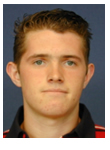
\includegraphics[width=1in,height=1.25in,clip,keepaspectratio]{Images/SchaepsTim.jpg}}]{Student 1}
Tim Schaeps received his M.S. in Applied Engineering: electronics-ict in 2007. Also in  2007 he started his Phd research on tomogaphy at the University of Antwerp.Lorem ipsum dolor sit amet, consectetuer adipiscing elit. Duis hendrerit sodales orci. Vivamus sed felis. Suspendisse consequat viverra sapien. Pellentesque habitant morbi tristique senectus et netus et malesuada fames ac turpis egestas. Suspendisse quis nulla. In pede. Nam tellus nisl, interdum vitae, lobortis et, faucibus at, lacus. Praesent nec quam. Pellentesque habitant morbi tristique senectus et netus et malesuada fames ac turpis egestas. Nunc condimentum quam vitae nisi. Fusce elit justo, venenatis in, vulputate a, hendrerit et, eros. In eget enim a nisi congue interdum. 
\end{IEEEbiography}
\begin{IEEEbiography}[{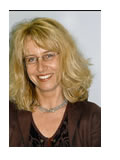
\includegraphics[width=1in,height=1.25in,clip,keepaspectratio]{Images/GoossensMaggy.jpg}}]{Student 2}
Lorem ipsum dolor sit amet, consectetuer adipiscing elit. Duis hendrerit sodales orci. Vivamus sed felis. Suspendisse consequat viverra sapien. Pellentesque habitant morbi tristique senectus et netus et malesuada fames ac turpis egestas. Suspendisse quis nulla. In pede. Nam tellus nisl, interdum vitae, lobortis et, faucibus at, lacus. Praesent nec quam. Pellentesque habitant morbi tristique senectus et netus et malesuada fames ac turpis egestas. Nunc condimentum quam vitae nisi. Fusce elit justo, venenatis in, vulputate a, hendrerit et, eros. In eget enim a nisi congue interdum. 
\end{IEEEbiography}

\vfill

% that's all folks
\end{document}


